\documentclass[a4paper]{article}
\usepackage{graphicx}
\usepackage{listings}
\usepackage{rotating}
\usepackage{subcaption}
\usepackage[export]{adjustbox}
\usepackage{hyperref}
\usepackage{amsmath}
%\usepackage[margin=1in]{geometry}
\begin{document}
\centerline{\Large \bf Individual Project - Interim Project Report}
\medskip
\centerline{\bf Alexander Lown}
\bigskip

%------------------------------------------------------------------------------
\section{Introduction}
I investigated the ability to automatically speed-up (or reduce power of) parts of existing applications, without a need to write custom offload hardware for each program, or even to re-compile; in a computing system with both conventional CPUs but also some configurable logic (FPGA fabric-like) area.

One such example of a computing system are the Xilinx Zynq series ICs, of which I have been working using a Zynq ZC702 development board, which contains a xc7z020 IC at its core. The xc7z020 IC contains a dual core ARM Cortex A9 'processor' (hereafter referred to as the PS) along with full MMU, DDR3 controller and APB peripherals (UART, Ethernet, SD, etc.), as well as a large programmable logic area based off a 28nm HKMG fabrication (hereafter referred to as the PL). A variety of AXI ports (and assosciated control signals such as user configurable clocks and interrupts) enabling communication between the PS and PL at high speed. Refer to figure \ref{fig:inter-block} for a detailed overview of how the PS and PL are interconnected. Whilst this is a quite specific system, there are strong parallels with a more conventional (as of the 2000s-2015s) PC, which could be supplemented with a PL card over PCI-E, in the same way that graphics tasks are offloaded to custom silicon in the form of a dedicated GPU, or more recent processing assistance designs such as the Xeon Phi.

This project uses the High Performance AXI controllers connected to some soft-IP performing DMA to enable the PL to interact directly with user-memory whilst running. Programs are run on top of Linux on the PS, rather than working only with bare metal enabling a significantly increased use-case. A kernel module (XDMA) grants user-space access to this DMA'd memory enabling any program to take advantage of it for offloading.

The project requires the existence of several connected fragments to work: the default HDL implementation, which is extended with HDL generated from analysis of the elf binary run on the PS in userspace (and optionally fed with profiling data to suggest blocks to preferrentially run on the PS, interacting through DMA using the kernel-exposed interface.

The project is designed currently to only work with basic blocks (BBs) which are sequences of instructions without any conditional, branching or jumping behaviour for simplicity. There is no reason it would not be possible to add support for these constructs in further work.

\begin{figure}[p]
  \includegraphics[width=1.4\textwidth,center]{fig/interconnect-block.eps}
  \caption{Xilinx UG585 Figure 5-1: Interconnect Block Diagram}
  \label{fig:inter-block}
\end{figure}

%------------------------------------------------------------------------------
\section{Background}
  \subsection{Initial State Investigation}

  I investigated the existing behaviour of the Zynq ZC702 development board using a variety of metrics in several situations, which will prove useful for Phases 2 and 3.
  This report will present an overview of the collected data, and will draw some conclusion for baseline behaviour.\\
  I have used 2 different benchmarks - the VTR 'basic' regression tests, and the encoding of a 10 second clip of 1280x720 resolution video (from Sintel) from YUV (y4m variant) to h264 using the x264 project.
  The choice of this second benchmark is related to one of the 'proposed' end-cases for this research project - namely hardware offloading of video encoding without the need for the encoder to be specifically written to target the Zynq PL.\\
  The collected data includes runtime, power, current, voltage and temperature information from the on-board PMICs, as well as system memory usage. The PS supports 3 speed steps (222MHz, 333MHz and 667MHz), but due to limitations of the peripheral clocks, only the latter two steps are valid states for testing.

\subsubsection{VTR}
  \paragraph{Runtime}
    Table \ref{tab:vtr:rt} shows the runtime for the various PS clock speeds.
    \begin{table}[tbp]
      \centering
      \begin{tabular}{l | l}
        Speed/MHz & Runtime/s \\
        \hline
        333 & 645 \\
        667 & 343 \\
      \end{tabular}
      \caption{Runtime vs Speed of PS for VTR}
      \label{tab:vtr:rt}
    \end{table}
    This suggests that halving the clock speed does not quite double the actual runtime. I propose that this is due to a reduction in the number of clocks spent idling on memory accesses, resulting in a more efficent usage of each clock cycle.

  \paragraph{Power}
    Figures \ref{fig:vtr:pow:667} and \ref{fig:vtr:pow:333} shows the 'power' as reported by the onboard PMIC for the VCCPx rails (power the PS) and VCCADJ rail (powers the DDR3 memory ICs and the corresponding IO banks).
    \begin{figure}[p]
      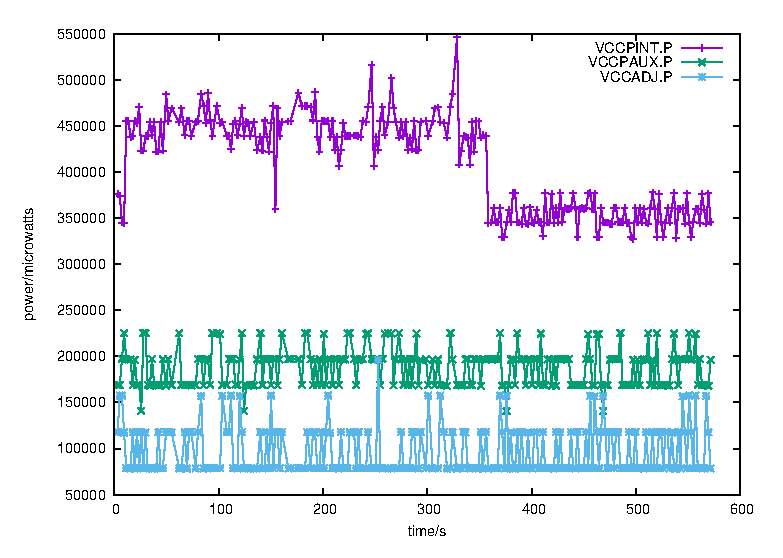
\includegraphics[width=\textwidth]{data/fig/vtr:pow:667.eps}
      \caption{Power usage of VTR at 667MHz}
      \label{fig:vtr:pow:667}
    \end{figure}
    \begin{figure}[p]
      \includegraphics[width=\textwidth]{data/fig/vtr:pow:333.eps}
      \caption{Power usage of VTR at 333MHz}
      \label{fig:vtr:pow:333}
    \end{figure}
    There is a clear uptick in VCCPINT usage after the first 4 samples, which is when the test is started. There is a large deviation in VCCPINT draw over the course of the benchmark at 667MHz, but a signifcantly reduced deviation when run at 333MHz - which I propose is due to the fewer stalls of the processor on memory accesses. On the other hand, VCCADJ's power usage at 333MHz is consistently higher, whilst at 667MHz, it peaks briefly but then returns to baseline for a much longer time - a behaviour I suggest follows on from it being able to complete trannsfers in a shorter time at the higher clock rate, enabling it to return the memory bus to idle sooner.

  \paragraph{Memory}
    Figures \ref{fig:vtr:mem:667} and \ref{fig:vtr:mem:333} show system memory usage for active pages, anonymous pages and the total committed address space during the running of the VTR tests.
    \begin{figure}[p]
      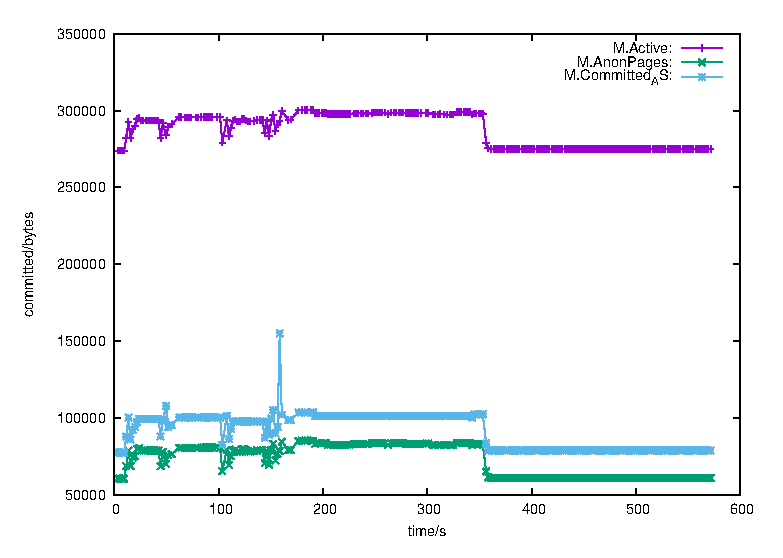
\includegraphics[width=\textwidth]{data/fig/vtr:mem:667.eps}
      \caption{Memory usage of VTR at 667MHz}
      \label{fig:vtr:mem:667}
    \end{figure}
    \begin{figure}[p]
      \includegraphics[width=\textwidth]{data/fig/vtr:mem:333.eps}
      \caption{Memory usage of VTR at 333MHz}
      \label{fig:vtr:mem:333}
    \end{figure}
    These show the allocated of anonymous pages for VTR (and its assosciated tools) to run in. The profiles are pretty similar during both sets of tests, due to changing the speed having little effect on the amount of memory needed. The major spikes in committed address space correspond directly to sudden decreases in the number of active pages - possibly an effect of the deallocations having occurred but the address space not being marked as uncommitted until after the next set of allocations has occurred.

\subsubsection{x264}
  \paragraph{Runtime}
    Table \ref{tab:x264:rt} shows the runtime for the various PS clock speeds.
    \begin{table}[tbp]
      \centering
      \begin{tabular}{l | l}
        Speed/MHz & Runtime/s \\
        \hline
        333 & 122 \\
        667 & 62 \\
      \end{tabular}
      \caption{Runtime vs Speed of PS for x264 encoding}
      \label{tab:x264:rt}
    \end{table}
    Unlike the VTR benchmarks, the runtime is unaffected by the speed of the processor core, despite making heaving usage of NEON optimizations, the limitation is clearly elsewhere\ldots

  \paragraph{Power}
    Figures \ref{fig:x264:pow:667} and \ref{fig:x264:pow:333} shows the 'power' as reported by the PMIC for the VCCPx rails and VCCADJ rail.
    \begin{figure}[p]
      \includegraphics[width=\textwidth]{data/fig/x264:pow:667.eps}
      \caption{Power usage of x264 at 667MHz}
      \label{fig:x264:pow:667}
    \end{figure}
    \begin{figure}[p]
      \includegraphics[width=\textwidth]{data/fig/x264:pow:333.eps}
      \caption{Power usage of x264 at 333MHz}
      \label{fig:x264:pow:333}
    \end{figure}
    At 667MHz, there is an increase of 250mW on VCCPINT for the ~62 seconds, but for 333MHz, there is an increase of only 120mW for the 122 seconds, indicating that running at 333MHz consumes less power in total for the same task.

  \paragraph{Memory}
    Figures \ref{fig:x264:mem:667} and \ref{fig:x264:mem:333} show system memory usage.
    \begin{figure}[p]
      \includegraphics[width=\textwidth]{data/fig/x264:mem:667.eps}
      \caption{Memory usage of x264 at 667MHz}
      \label{fig:x264:mem:667}
    \end{figure}
    \begin{figure}[p]
      \includegraphics[width=\textwidth]{data/fig/x264:mem:333.eps}
      \caption{Memory usage of x264 at 333MHz}
      \label{fig:x264:mem:333}
    \end{figure}
    These show a fairly constant memory profile, occupying almost half of the total memory to encode 1280x544p footage.

  \paragraph{Profiling}
    The listings \ref{lst:x264:667} and \ref{lst:x264:333} show the gprof data collected from the benchmarked instances of x264.
    \begin{sidewaysfigure}[p]
      \lstinputlisting[firstline=4, lastline=20]{data/x264/vtr-gmount.out-667-profiled}
      \caption{gprof data for x264 at 667MHz}
      \label{lst:x264:667}
    \end{sidewaysfigure}
    \begin{sidewaysfigure}[p]
      \lstinputlisting[firstline=4, lastline=20]{data/x264/vtr-gmount.out-333-profiled}
      \caption{gprof data for x264 at 333MHz}
      \label{lst:x264:333}
    \end{sidewaysfigure}
    At 667MHz, \verb x264_me_search_ref is the main hotspot - due to lots of stalls on memory accesses, which don't stall at 333MHz - due to the 'reduced' latency the PS sees. At 333MHz, \verb x264_pixel_* routines take up the majority of the time, as these routines are performing lots of arithemtic computation on a few pixels. These look like ideal candidates to offload to the PL. A few of the \verb x264_pixel_* routines are shown in listing \ref{lst:x264:ass} to demonstrate.
    \begin{sidewaysfigure}[bp]
      \centering
      \begin{subfigure}[b]{0.45\textwidth}
        \lstinputlisting[firstline=805, lastline=825]{pixel-a.S}
        \caption{The saturation 8x8 calculations using NEON extensions}
      \end{subfigure}
      \qquad
      \begin{subfigure}[b]{0.45\textwidth}
        \lstinputlisting[firstline=401, lastline=417]{mc-a.S}
        \caption{The average (width 16) calculations using NEON extensions}
      \end{subfigure}
      \caption{ARM Assembly for some of the pixel routines from x264}
      \label{lst:x264:ass}
    \end{sidewaysfigure}

    Further investigation of these results showed that they were not as optimal candidaes for offloading as initially suggested, due to the encoding process at the default levels spending too much time in memory accesses, rather than in pure-computational work. As such the profiling data was re-run with higher quality encoding presets of x264. I chose to try use the presets 'slower', 'very slow' and 'placebo'. An overview of the result can be seen in table \ref{tab:x264:prof-extra} and listings \ref{lst:x264:slower}, \ref{lst:x264:very-slow} and \ref{lst:x264:placebo}.

    \begin{sidewaystable}[tbp]
      \centering
      \begin{tabular}{l | p{12cm} | l | l}
        Profile & Equated Flags & Average FPS & Runtime/s \\
        \hline\\
        slower & --b-adapt 2 --direct auto --me umh --partitions all --rc-lookahead 60 --ref 8 --subme 9 --trellis 2  & 0.55 & 190\\
        very-slow & --b-adapt 2 --bframes 8 --direct auto --me umh --merange 24 --partitions all --ref 16 --subme 10 --trellis 2 --rc-lookahead 60 & 0.30  & 347\\
        placebo & --bframes 16 --b-adapt 2 --direct auto --slow-firstpass --no-fast-pskip --me tesa --merange 24 --partitions all --rc-lookahead 60 --ref 16 --subme 11 --trellis 2  & 0.06 & 1733 \\
      \end{tabular}
      \caption{Runtime and Flags for more difficult x264 settings}
      \label{tab:x264:prof-extra}
    \end{sidewaystable}

    \begin{sidewaysfigure}[p]
      \lstinputlisting[firstline=4,lastline=20]{data/x264/x264-slower.gprof}
      \caption{gprof data for x264 using 'slower'}
      \label{lst:x264:slower}
    \end{sidewaysfigure}
    \begin{sidewaysfigure}[p]
      \lstinputlisting[firstline=4,lastline=20]{data/x264/x264-very-slow.gprof}
      \caption{gprof data for x264 using 'very-slow'}
      \label{lst:x264:very-slow}
    \end{sidewaysfigure}
    \begin{sidewaysfigure}[p]
      \lstinputlisting[firstline=4,lastline=20]{data/x264/x264-placebo.gprof}
      \caption{gprof data for x264 using 'placebo'}
      \label{lst:x264:placebo}
    \end{sidewaysfigure}

    These show quite a different picture to the default profile, we can see a large quantity of PS time (and power) being spent in functions such as \verb x264_pixel_ads{14} which are entirely arithmetic, along with the NEON optimized \verb x264_pxel_sad_x3_*_neon functions. This suggests that x264 is definitely still a good use case for which PL-backed offloading could result in increased performance, as opposed to simply power reduction.

  \subsection{Work Completed Currently}
  Due to the large area of interaction required to make this project complete, there has been work on programs in Linux user space, Linux kernel space, and HDLs (VHDL, Verilog and IP block design), utilizing a variety of tools and languages.

  I could include large quantities of this as part of the report, but will chose instead to include only small snippets and point the reader to the Github repositories if they are interested in the full code bases, with all the supporting scripts and build systems - though I warn them that there is ~20-30GB of both proprietary and free tools required to recreate results.

  The currently relevant code bases can be found at \url{https://github.com/alown/zynq}, \url{https://github.com/alown/zynq-xdma} and \url{https://github.com/alown/vtr}.

  Some of the main files (the more interesting ones) are described briefly below:

  In the zynq repository:

  \verb elf/analysis.rb  is a Ruby script that performs offline arm elf binary analysis involving splitting the application into BBs, then performing analysis looking for BBs with a high density of easily offloadable arithmetic instructions, and high density of NEON instructions. It is also able to emit VHDL for many of ARMs 'data-processing' instructions (including support for shifted register operands), as well as the 4 standard MUL variants. This VHDL acts like a 'fused instruction' for the entirety of the parallelizable section of the BB. The effectiveness of this depends entirely on the data dependencies in the BB under consideration. This VHDL fits into the \verb offload.vhdl  file.

  \verb elf/offload.vhdl  is a simple wrapper entity for the generated VHDL that presents some signals representing the r0-r13 registers.
  \verb elf/offload-top.vhdl  presents an AXI4-S (AXI-4 streaming) interface to unpack/pack the starting/end values for r0-r13 for the offload block, as well as coordinating everything using a simple FSM.

  The Vivado Project \verb tmp/vivado/[\ldots]simple.xpr  holds together all of the generated offloaded code by linking it to the rest of the system using Xilinx DMA IP over the HP0 AXI port described earlier, and shown in figure \ref{fig:inter-block}. A high-level block diagram showing the interactions between the offloaded code (shown as the \verb addtest  IP block), and the rest of the design can be found in figure \ref{fig:vivado-block}.

  \begin{sidewaysfigure}
    \centering
    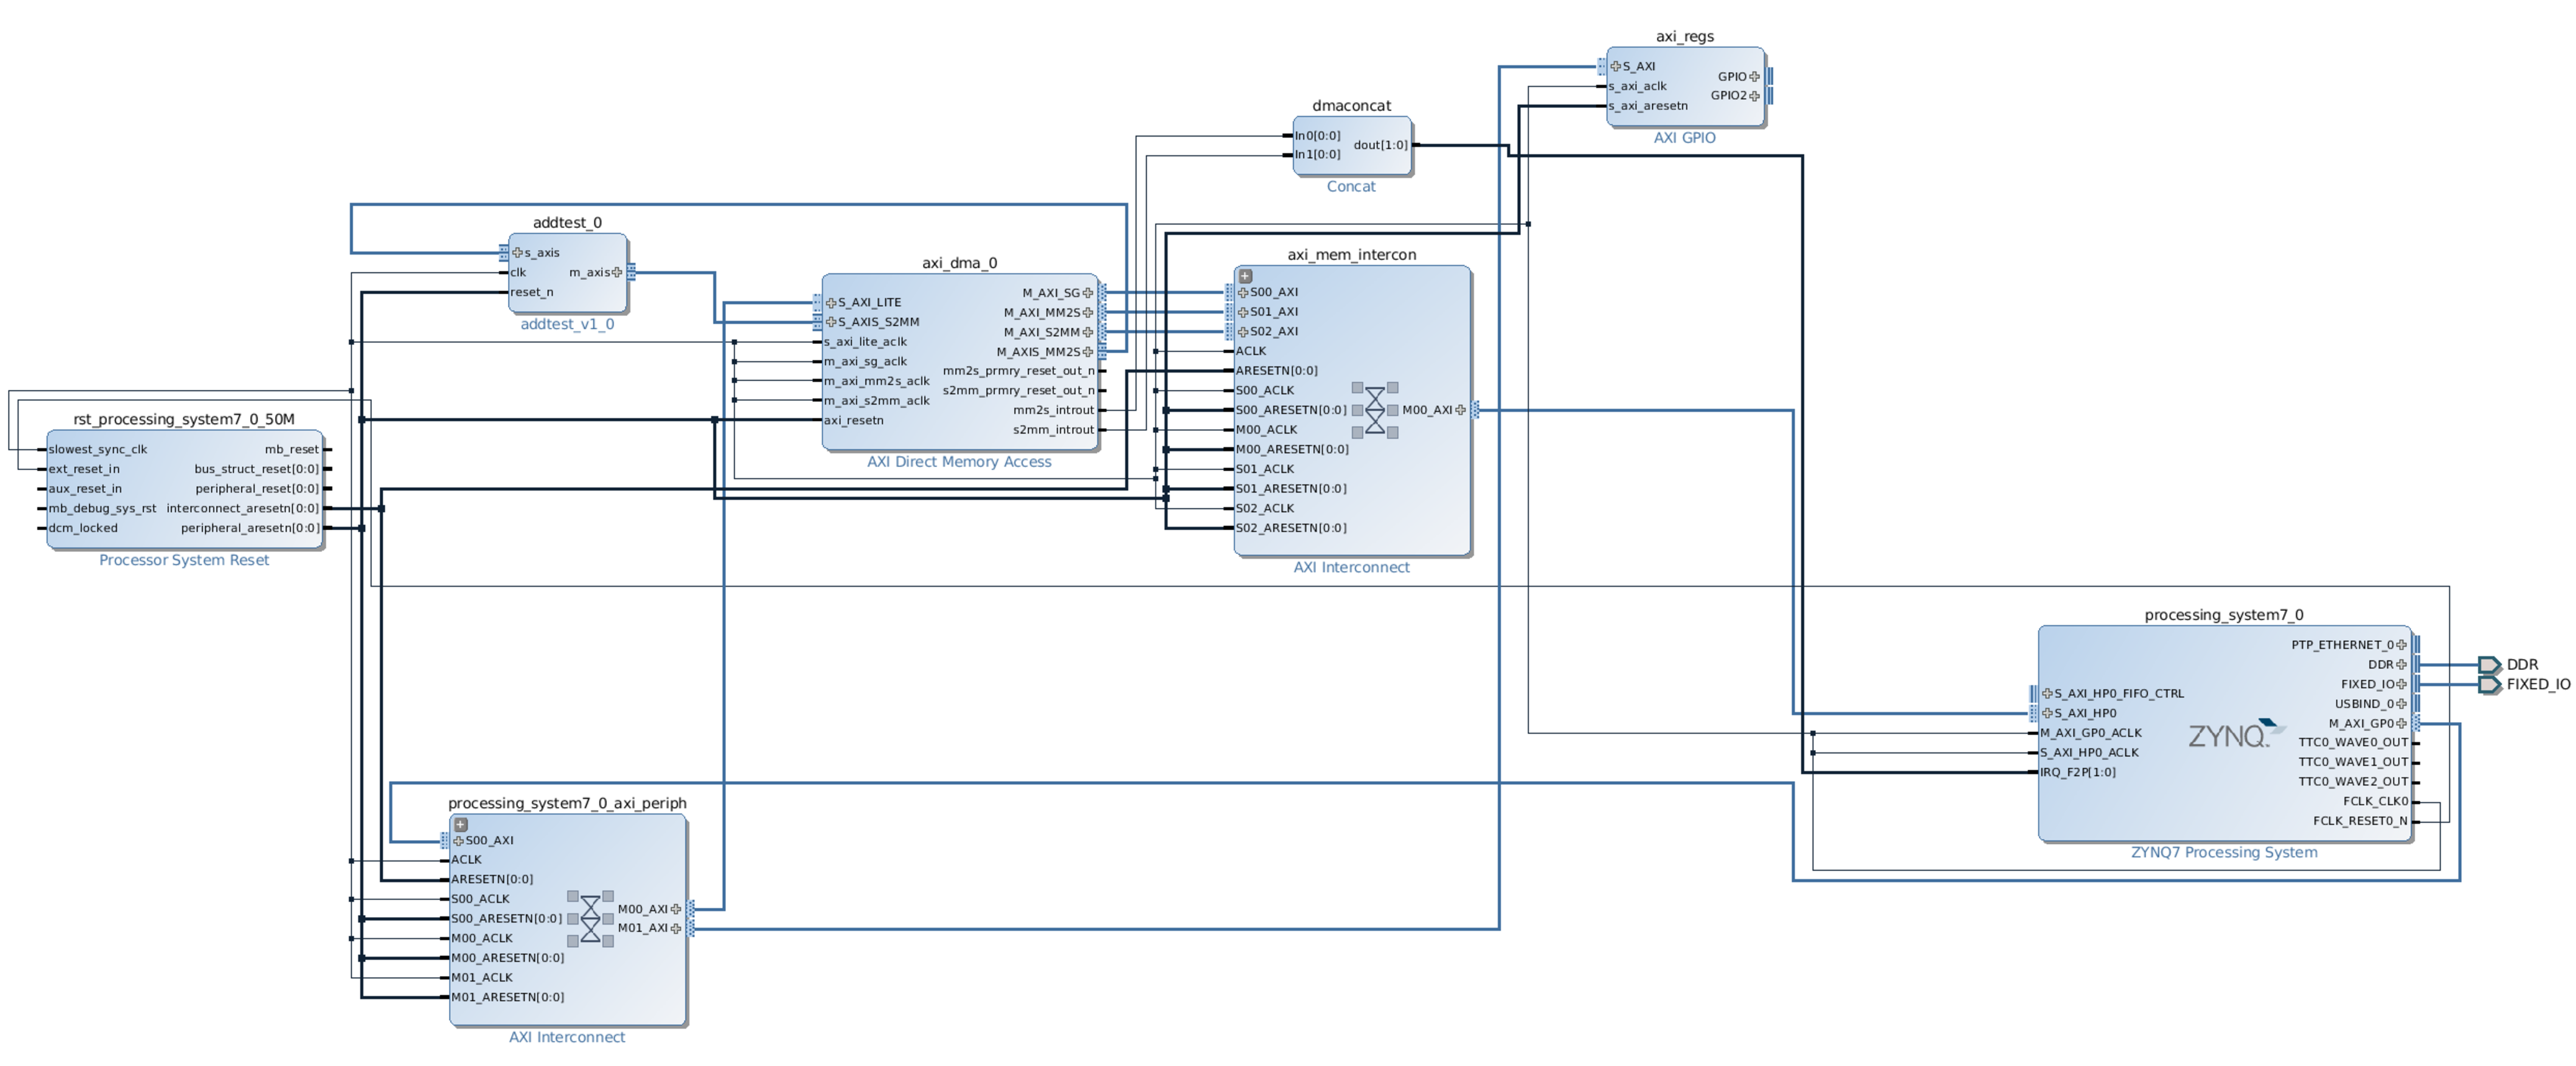
\includegraphics[width=\textwidth]{fig/vivado-block.eps}
    \caption{Vivado Block Design}
    \label{fig:vivado-block}
  \end{sidewaysfigure}

  To avoid spending unnecessary time writing and debugging a Linux kernel module to do DMA, I have chosen to extend from an existing project called XDMA, which presents the DMA IP as a block device at \verb /dev/xdma . The XDMA project also came with a simple user-space shared library to make adding support to a new application as easy as linking to the shared library and the transfer function at appropriate times.

  I verified the functionality of the PL DMA IP, and the whole userspace stack by originally connected the design with a 1024 deep FIFO over the AXI4-S interface, which then let me perform simple write/wait/read tests from userspace to verify a lack of corruption and to get an idea of the speed of such transfers.
  A DMA transfer to/from the FIFO of a $32\text{bit} * 1024 = 4096\text{bytes}$ was able to achieve speeds of ~$190\text{MB/s}$ using an in-PL clock of $150\text{MHz}$.

  In the zynq-xdma repository:

  \verb demo/xdma-offload.c  is a small user-space testing program which performs the required packetization of some possible register values, then transfers to the PL to do work, then reads the resulting register values back out of the DMA engine and prints it back to the user for verification.

%------------------------------------------------------------------------------
\section{Project Plan}
The project has several areas to be completed prior to exploring extensions such as decreasing the amount of processing required, or optimizing the HDL tools.

Currently only a small number of ARM instructions have rules governing their transliteration to valid HDL, which are the simple data-processing instructions such as ADD, MOV, MUL, etc, adding support for a larger section of the instruction set would allow for benchmarking using VTR and x264, to allow comparison with the initial data, as currently only some small custom-written test cases using the limited available instructions are offloadable.
One of the areas which is expected to provide large performance improvements (as these generally indicate the hotspots in the application), are the BBs utilizing NEON instructions, so implementing support for transliterating these to HDL is likely to result in significant measurable changes, as it allows us to effectively create instructions based on fusing a whole BB together (notwithstanding data dependency restrictions).

Currently each BB that is offloaded has the overhead of being a DMA write of the starting conditions of the registers, along with a DMA read of the end results, before feeding these back into the PS to perform the conditional/branch. Adding support for detecting short branches indicative of loops would allow the whole loop to be offloaded (and in some cases unrolled onto logic) allowing for possible speed ups.

Currently BBs (as defined for this project) exclude any loading/storing of results as the PL lacks the ability to perform the required VADDR $\rightarrow$ PADDR lookups that the Linux kernel handles for the application. This could be worked around in some situations by pre-fetching all the data to be loaded, and then transferring this to the PL, which can then perform the required work, along with keeping track of any stores it 'performs' the results of which can be transferred back to the PS before being performed from there.

Currently the analysis of a given application is required to be run in advance (along with any runs to gather profiling data), which then generates HDL to be fed into Xilinx's toolsuite to generate a new bitstream for programming. The analysis can take 30 or more seconds for larger applications, along with consuming multiple gigabytes of RAM as it keeps copies of every basic block it finds in memory, before culling them by determing whether they are 'interesting' to offload based upon the amount of arithmetic operations performed, or the amount of NEON instructions performed (particularly sequentially).

%------------------------------------------------------------------------------
\section{Evaluation Plan}
As this project is interested in the use of processing systems with PL for offloading, any overhead time caused by the running of the HDL toolsuite should be excluded from benchmark results.

The project is able to optimize for two different cases: increased speed or increased power efficency, and may be unable of optimizing more efficently than simply running the application on the PS could yield for certain use cases. Benchmarking for the exact application there is interest in is definitely required, as different binary outputs are likely to result in the analysis program finding different suitable arears to offload (or maybe even none at all).

The project is interested in being a feasibility study through a trial implementation, rather than necessarily being an immediately useful product, so it is possible the conclusion may yield this as a dead end until further research elsewhere.
%---------------


\end{document}
